
\section{Architecture Logiciel}

Nous avons divisé notre modèle en trois grandes architectures, le serveur, la machine d'états et les unités.

\subsection{Architecture du serveur}

TODO: Expliquer l'architecture du serveur en détail, c'est-à-dire 2 listes: une de player et une de sockets, il y a une stateMachine qui gère les différents états du jeu,
le jeu est créé quand les 2 joueurs sont connectés, la carte est envoyée à  ce moment-là, quand une action est effectuée qui change la carte il faut renvoyer la carte

\subsection{Architecture de la machine d'états}
\begin{figure}[H]
    \centering
    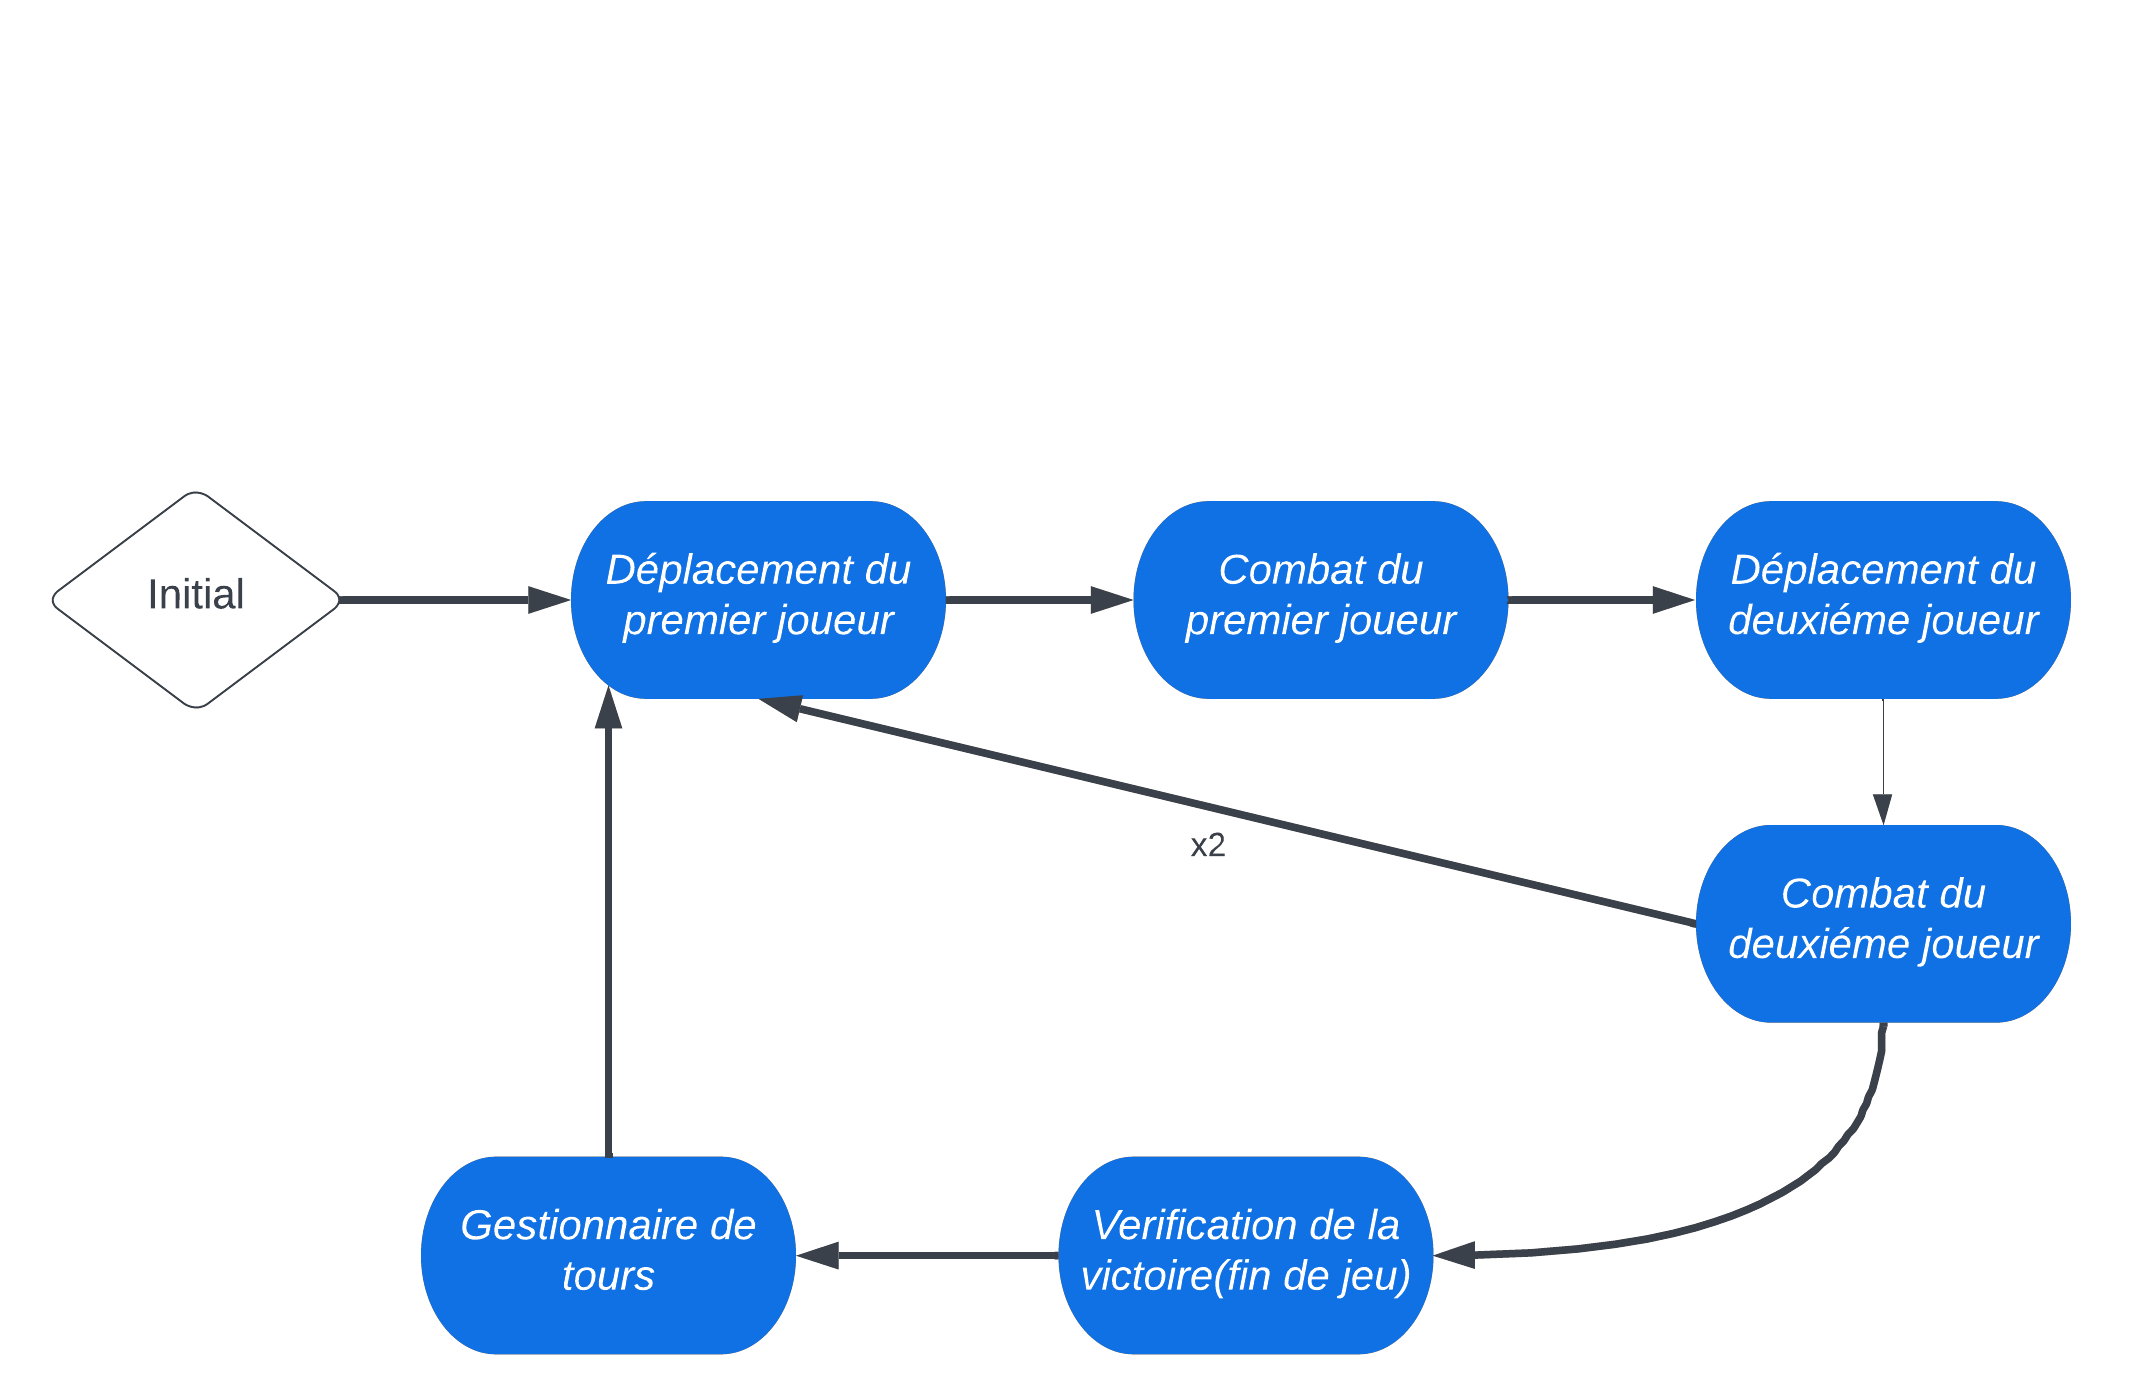
\includegraphics[scale=0.2]{data/State_Machine.png}
    \caption{Schéma de la machine d'état implémentée}
    \label{fig:schema_state_machine}
\end{figure}

Le schéma de l'automate dans la figure ci-dessus est une version simplifiée de notre automate, car, comme vous pouvez le voir, elle contient une transition x2, qui signifie la répétition des 4 premières phases une autre fois pour chaque tour, ce qui est exigée dans les règles.

Nous avons décidé de supprimer plusieurs phases à cause du manque du temps. Ces phases sont : la phase des événements spéciaux, car elle était très compliquée à implémenter, la phase de la supériorité aérienne, car nous n'avons pas implémenté les unités aériennes, la phase de renforts, car nous n'avons pas eu le temps d'implémenter une tactique de renfort, la phase d'allocation, car nous avons fait en sorte que les joueurs ont qu'une seule base, et cette phase servait principalement pour l'activation de plusieurs bases, la phase d'initiative, car nous avons fait en sorte que l'ordre de jeu ne change pas entre tours et finalement la phase de supply attrition, car nous faisons déjà ce qu'elle est censée faire a chaque début de phase de mouvement.

Cela laisse finalement 10 phases en total, dont la phase de mouvement du premier joueur, la phase de combat du premier joueur, le phase de mouvement du deuxième joueur et la phase de combat du deuxième joueur se répètent 2 fois, car c'est exigé que dans un tour il faut qu'un joueur puisse bouger ses unités et attaquer deux fois. Ensuite nous avons la phase de vérification de fin de jeu(ou de la victoire), qui vérifie si le nombre de tours dépasse 38, dans ce cas le premier joueur gagne, ou si un des joueurs a perdu toutes ses unités, et dans ce cas, le joueur avec des unités restantes gagne. La dernière phase est la phase du gestionnaire de tours, qui met simplement à jour le nombre de tours en augmentant par 1 le nombre du tour actuel.

Nous utilisons cette machine d'état pour gérer toutes les commandes du jeu, pour vérifier les approvisionnements des unités, pour savoir si le joueur peut effectuer une action dans cette phase, etc. Nous avons donc une machine d'état qui permet de gérer essentiellement tout le jeu, vu que ce dernier dépend complètement de cette machine d'état.


\subsection{Architecture des unités}

\begin{figure}[H]
    \centering
    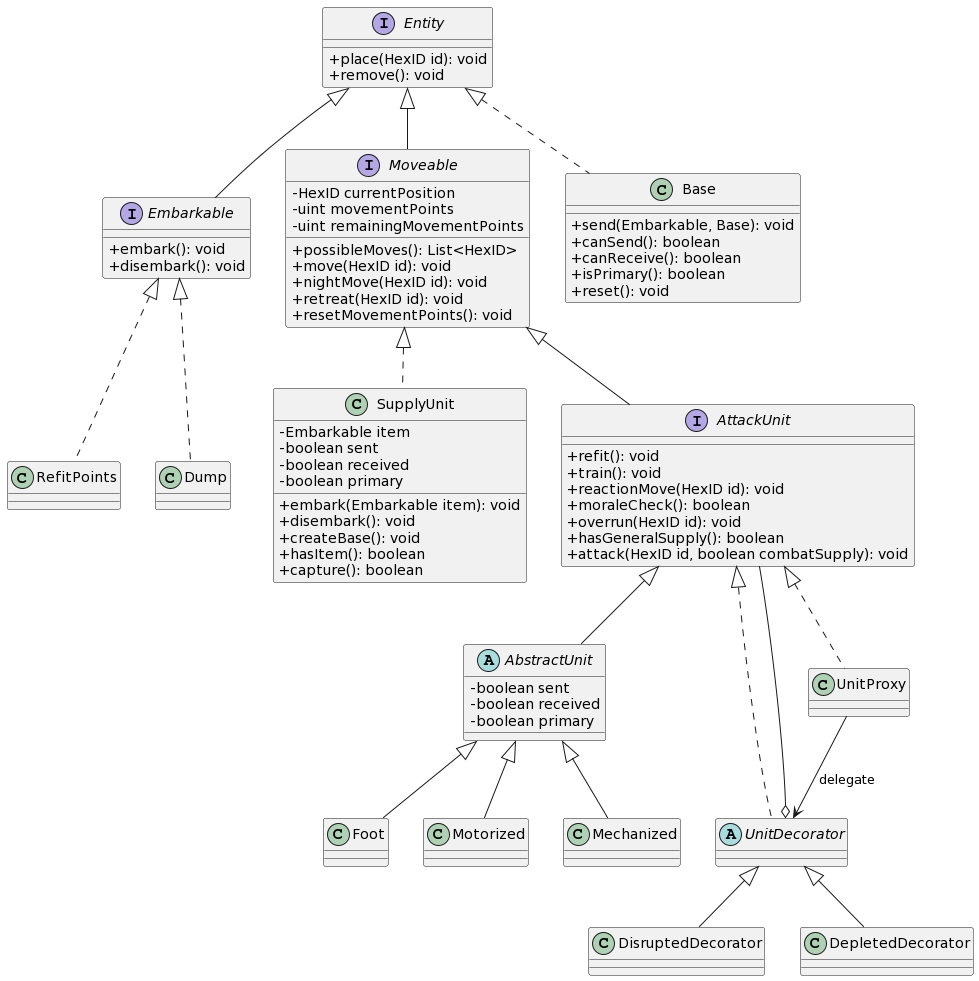
\includegraphics[scale=0.3]{data/uml_entityV4.png}
    \caption{Diagramme UML de l'objet Entity}
    \label{fig:uml_entity}
\end{figure}

Nous avons fait le choix de réunir toutes les unités sous la même interface, ce qui nous permet d'avoir un seul type pour toutes les unités et donc de pouvoir faire des listes de ces entités dans la partie serveur.
Pour une meilleure factorisation on sépare les unités en deux, celles qui peuvent bouger (\lstinline{Moveable}) et les autres. Nous séparons de nouveau en unités de soutien et d'attaque. Pour assurer la maintenance du code et rajouter des fonctionnalités, nous avons utilisé deux designs patterns, le \lstinline{Decorator} et le \lstinline{Proxy}. Mais pour pouvoir utiliser ces patterns nous avions la contrainte suivante, il fallait que les deux patterns implémentent une interface comme montrer ci-dessous. Nous avons donc était forcé d'ajouter une interface intermédiaire (ici \lstinline{AttackUnit}) pour pouvoir les implémenter. Le décorateur nous permet de changer le comportement des unités dynamiquement sans à avoir à changer toutes les classes qui étendent \lstinline{AbstractUnit}. Mais l'utilisation de ce pattern conduit à un problème, on peut appliquer un décorateur à un objet déjà décorer un nombre de fois infinie. Ce qui nous amène donc à utiliser un \lstinline{Proxy} qui permet de contrôler l'utilisation du décorateur.

Toute la démonstration précédente était notre réflexion lors de la conception de l'architecture. Mais nous avons implémenté l'attaque en dernier, nous n'avons donc pas intégré ces patterns dans notre code.

\begin{figure}[H]
    \centering
    \def\stackalignment{r}
    \stackunder{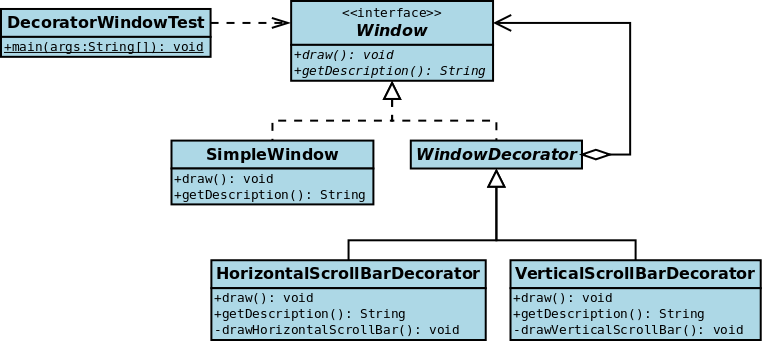
\includegraphics[scale=0.3]{data/UML_Decorator_Pattern_Example.png}}%
    {\scriptsize%
        Source : Wikipédia}
    \caption{Exemple d'un {\tt Decorator}}
    \label{fig:UML_Decorator_Pattern_Example}
\end{figure}


\begin{figure}[H]
    \centering
    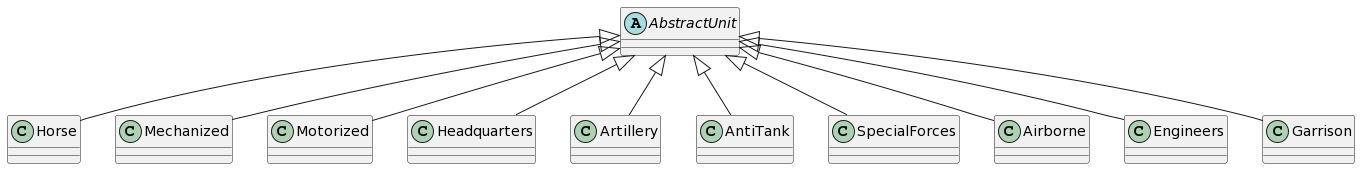
\includegraphics[scale=0.3]{data/uml_abstract_unit.png}
    \caption{Diagramme UML des unités}
    \label{fig:uml_abstract_unit}
\end{figure}

Dans les règles, il existe toutes les unités d'attaque qui se trouvent ci-dessus. Comme nous avions un temps limité nous avons décidé de ne pas toutes les implémenter, car même si certaines ont un comportement différent le travail aurait été trop chronophage et donc nous avons privilégié des aspects plus importants du projet. On peut trouver les unités d'attaque choisies dans le diagramme \ref{fig:uml_entity} (Foot, Mechanized, Motorized).

\subsection{Mouvement et Approvisionnement}

Un des mécanismes principaux du jeu est le mouvement des unités.
Sur une carte composée d'hexagones, une unité peut se déplacer si certaines conditions sont satisfaites.
Par exemple, une unité ne peut pas avancer dans un hexagone avec des ennemis présents, ou si l'unité n'a plus de
points de mouvement, une valeur numérique que chaque unité contient. Ayant débuté avec un mouvement simple (case
par case), nous avons implémenté l'algorithme de Dijkstra (que nous avons appris en cours d'algorithmique des graphes en Licence) 
avec nos propres modifications, pour bien l'intégrer dans
le contexte du jeu. En ayant comme entrée l'unité qui souhaite bouger et l'hexagone de destination, notre algorithme
crée un graphe à partir des hexagones de la carte, chacun étant un nœud du graphe et les connexions avec ses voisins
les arêtes du graphe.

Chaque hexagone contient son type de terrain (montagne, plaines, désert...), qui lui-même contient les points
de mouvements requis pour bouger dans celui-ci. Ceci est très utile dans le mouvement, pour trouver le plus court
chemin entre un hexagone A et un hexagone B. En commençant par l'hexagone ou se trouve l'unité, nous faisons un
parcours en largeur, en calculant le coût nécessaire pour bouger a chaque fois. Enfin nous retenons le plus court
chemin et puis nous appliquons le mouvement si l'unité a assez de points de mouvements. Les modifications sur
l'algorithme Dijkstra de base sont que nous vérifions si nous passons dans un hexagone contenant une unité ennemie,
ainsi que si nous passons à côté d'une unité exerçant une zone de contrôle, ce qui nous ralentit (augmente le coût
d'un hexagone). La zone de contrôle est un mécanisme du jeu ou chaque unité exerce une influence autour de son
hexagone. Donc tout hexagone adjacent de la position d'une unité se trouve dans sa zone de contrôle.
La seule exception ou une unité n'exerce pas de zone de contrôle est si l'unité a le statut de {\tt disrupted}.
Disrupted est un statut que toute unité peut avoir a un moment donné que nous expliquerons plus bas, et qui donne
des effets négatifs à une unité.

Un autre mécanisme lié fortement avec le mouvement est l'approvisionnement. Effectivement pendant une guerre,
approvisionner les unités est très important. Nous parlerons à partir de maintenant de l'approvisionnement en
tant que {\tt supply}, pour simplifier. Les supply peuvent se diviser en deux catégories, les {\tt general supply} et les
{\tt combat supply}. Une unité peut avoir les deux en même temps ou un seul, dépendant des conditions du jeu. De plus,
nous avons des caisses d'approvisionnement, les dénommés {\tt dump}. Les dump sont placés sur la carte et peuvent
être utilisés pour donner soit du general supply ou du combat supply a une unité. Nous avons ensuite des camions,
les unités de soutien, qui peuvent emporter des dump et quelques unités spécifiques, pour les déplacer et déposer
rapidement sur la carte. Enfin, chaque joueur a des bases pour organiser son approvisionnement, placés, elles aussi,
sur la carte.

Pour définir si une unité a du general supply, il faut pouvoir tracer un chemin depuis l'unité, jusqu'au dump ou la
base amie la plus proche. Ce chemin peut être de longueur 7 au maximum jusqu'à un dump, ou 14 jusqu'à une base. Par
contre, ce chemin peut être étendu, si une unité de soutien se trouve sur ce chemin. Si c'est le cas alors le chemin est
étendu de 7 hexagones. Par exemple, si une unité A est à une distance de 20 hexagones d'une base B, alors normalement
il n'y a pas de chemin pour pouvoir bénéficier de general supply. Si par contre, il existe une unité de soutien entre
A et B, alors nous pourrons tracer un chemin grâce à l'extension de la distance que l'unité de soutien nous donne.
Pour faire ça en réalité, nous avons conclu que la logique ressemblait beaucoup à notre algorithme de mouvement,
avec des contraintes en plus. Nous avons donc modifié notre algorithme de Dijkstra pour pouvoir l'utiliser dans
le cas où nous voulons tracer un chemin entre une unité et un dump ou une base. Enfin, il fallait ajouter dans ce cas, comme le fait que nous ne pouvons pas tracer un chemin qui passe par des montagnes,
ou par une zone de contrôle ennemie.

Pour connaître si une unité a accès au combat supply, il suffit de suivre les étapes que pour le general supply,
mais en excluant les bases, car une unité peut obtenir des combats supply seulement depuis un dump.

Ne pas avoir un des types de supply peut avoir des effets dévastateurs sur une unité. Si au début de la phase de
mouvement une unité ne peut pas tracer un chemin pour avoir du general supply, alors elle est disrupted.
Dans ce cas, l'unité ne peut pas exercer de zone de contrôle, son mouvement est réduit de moitié et l'unité est
moins bonne au combat. Si l'unité n'a pas de combat supply, alors elle est moins bonne au combat, ce qui sera plus
détaillé dans la partie où nous expliquons le déroulement du combat.

\subsection{Combat}

Le combat était la partie du moteur de jeu la plus compliquée à implémenter.
Il fallait combiner plusieurs tableaux complexes avec des relations très spéciales entre eux.
Ceci bien sûr pour ordonner à des unités dans un hexagone d'attaquer des unités ennemies dans un hexagone adjacent.
Nous pouvons voir ci-dessous le tableau fourni dans les règles du jeu :

\begin{figure}[H]
\centering
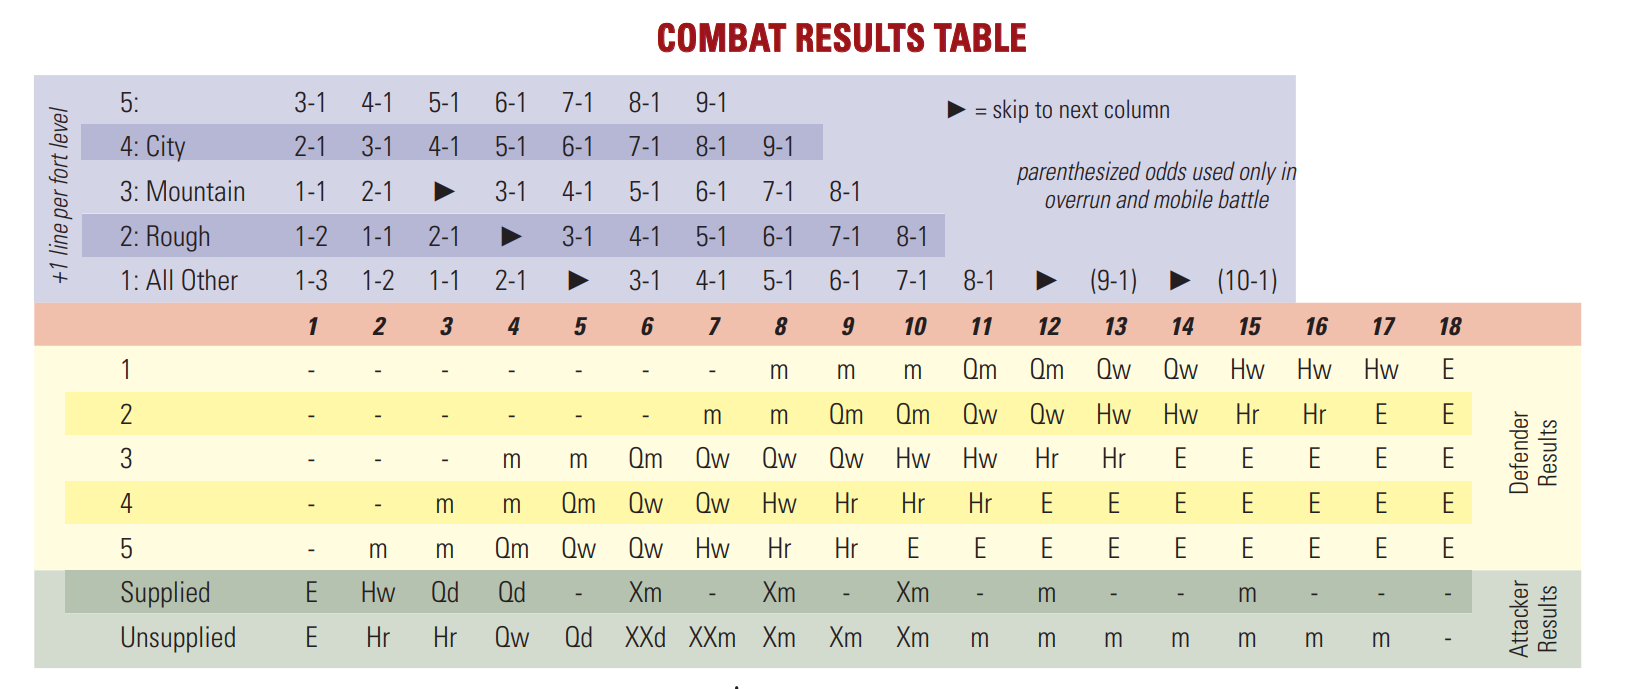
\includegraphics[scale=0.25]{data/tableau_combat.png}
\caption{Tableau du combat}
\end{figure}

Pour interpréter ce tableau, il faut le diviser en trois parties distinctes. En haut la partie en bleu est la première étape.
Nous choisissons la ligne correspondant au type de terrain de l'hexagone que nous attaquons, puis on divise le nombre
d'attaquants par le nombre de défenseurs présents dans l'hexagone cible. Avec ce ratio, nous choisissons ensuite la colonne.
Ensuite nous passons à la deuxième partie du tableau, en rouge et jaune. Avec le ratio que nous avons trouvé avant,
nous trouvons quelle colonne rouge correspond. On lance un dé (1d6) et on ajoute le résultat pour trouver la colonne finale.
Si par exemple nous étions sur la colonne 5 et le dé retourne 3, nous nous déplaçons sur la colonne 8.
Enfin pour choisir la ligne, nous prenons la valeur morale Rating de chaque défenseur, pour trouver la case correspondante.
Morale Rating est un attribut que chaque unité contient. Plus elle est petite, plus l'unité performe bien en combat.
Avec la case trouvée, on récupère deux lettres distinctes. La première représente le résultat des dégâts subits et la deuxième le résultat du moral.
Si {\tt m} est seulement présent alors le résultat des dégâts est inexistant, et si {\tt E} alors le résultat du moral est inexistant.
Une barre signifie qu'il n'y a aucun résultat. Ces résultats sont pour les défenseurs.
Pour les attaquants, nous passons sur la dernière partie du tableau, la partie verte.
Nous gardons la même colonne qu'avant, et choisissons la ligne en dépendance de l'approvisionnement de l'attaquant.
S'il est approvisionné alors nous choisissons la ligne de haut, sinon la basse. Et récupère les résultats comme dans le cas des défenseurs.
Voici un petit tableau qui montre les résultats possibles :

\begin{figure}[H]
\centering
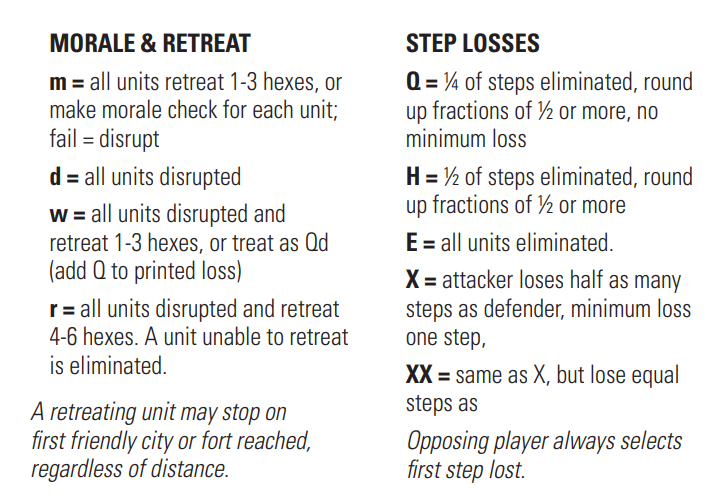
\includegraphics[scale=0.3]{data/morale_et_retraite.png}
\caption{Tableau des résultats de combat}
\end{figure}

Prenons un exemple pour mieux comprendre. Une unité A attaque une unité B. Le terrain de l'hexagone ou se trouve l'unité B est Rough, donc la ligne du tableau bleu est la deuxième.
Le ratio attaquants-défenseurs est de 1-1, car nous avons une seule unité A qui attaque une seule unité B. La colonne du tableau est alors 2.
Nous lançons un dé et le résultat est 3, donc la colonne finale est 5. Supposons que la valeur morale Rating de B est 3.
La valeur qui correspond est {\tt m}. Ceci veut dire que nous devons faire un test de morale.
Pour faire ceci nous lançons un autre dé et nous ajoutons la valeur morale Rating au résultat. Si le résultat est plus grand que 5, le test échoue.
Dans notre cas, le résultat est 4 et rien ne se passe. Passons aux combattants, qui dans ce scénario
n'ont pas d'approvisionnements. La valeur de la colonne 5 pour la ligne Unsupplied est {\tt Qd}.
Donc l'unité A reçoit un quart (arrondies) de ces points de vie en dégâts et A devient {\tt disrupted}.
Supposons que A a 1 point de vie, l'arrondie de 1/4 est de 0 donc l'unité ne reçoit pas de dégât.
Avec le statut {\tt disrupted} par contre, sa valeur de morale Rating augmente de 1 et A ne pourras bouger que la moitié de son mouvement pour le reste du tour.

\section{Technologies}

\subsection{Service d'hébergement}

Pour le service d'hébergement, nous avons utilisé le GitLab du CREMI comme demandé dans les consignes. Nous avons paramétré les pipelines pour qu'à chaque commit, il effectue les tests automatiquement pour aider à ne pas faire des commits complètement erronés.
Si les tests ratent, alors un mail est envoyé à l'auteur du commit et le commit est marqué sur GitLab avec une croix rouge signifiant l'échec des tests Concernant les branches nous avons divisé le dépôt en quatre :
\begin{itemize}
    \item main
    \item dev
    \item backend
    \item frontend
\end{itemize}

Le principe de base était que nous développions sur les branches (\lstinline{frontend} et \lstinline{backend}) puis que nous fusionnions ces deux dernières sur la branche \lstinline{dev}. A partir de là, nous vérifions que le frontend et le backend fonctionnaient bien ensemble. Si il avait une erreur, alors c'était là que nous travaillions en attendant de régler le problème. Une fois que nous avions une version stable, nous fusionnions la branche \lstinline{dev} à la branche \lstinline{main}. La branche main est réservée aux versions stables qui compilent et qui fonctionnent correctement. Malheureusement nous nous sommes vite rendu compte que ce n'était pas le moyen le plus optimisé de travailler, car lorsqu'on travaille sur la communication client-serveur sur le \lstinline{backend} et le \lstinline{frontend}, il fallait fusionner les deux branches sur la branche \lstinline{dev} pour pouvoir tester, ce qui prenait beaucoup de temps et était plutôt fastidieux. Nous avons décidé de travailler sur la branche \lstinline{dev} pour faciliter les tests de la communication client serveur. Il aurait sûrement fallu faire des branches en fonction des {\tt features}.

\subsection{Langage de programmation}

Nous avons choisi comme langage de programmation \lstinline{TypeScript} pour le \lstinline{backend} et le \lstinline{frontend}. En effet, en ayant la même technologie pour tout le projet cela rend la communication beaucoup plus simple entre les deux côtés. On aurait aussi pu utiliser \lstinline{JavaScript}, mais une surcouche de typage nous permet de sécuriser la production du code grâce à la vérification du typage à la compilation, qui n'existe pas dans \lstinline{JavaScript}. Enfin ce choix nous a laissé la liberté de ne pas faire que de la programmation objet, par exemple le \lstinline{frontend} est en majorité de la programmation impérative et fonctionnelle.

\subsection{Communication client-serveur}

Au départ nous étions parti sur une architecture avec un serveur web qui communiquait avec les clients grâce à des requêtes web HTTP.

Malheureusement cette architecture n'était pas adaptée pour un jeu de ce type puisque au moment où un joueur joue un coup, l'autre joueur doit être notifié de ce changement. Or si on utilise un serveur web HTTP le client devrait faire une requête au serveur pour être mis au courant, ce qui n'est pas pratique.

Pour un changement en direct sans faire une boucle de requêtes continuelles, il faudrait un système où le serveur peut envoyer un message au client sans requête au préalable.

C'est pour cela qu'une architecture avec des web sockets a été la solution que nous avons choisie.
Cette architecture permet d'envoyer des messages ou des données aux clients sans requête préalable.


\begin{figure}[H]
    \centering
    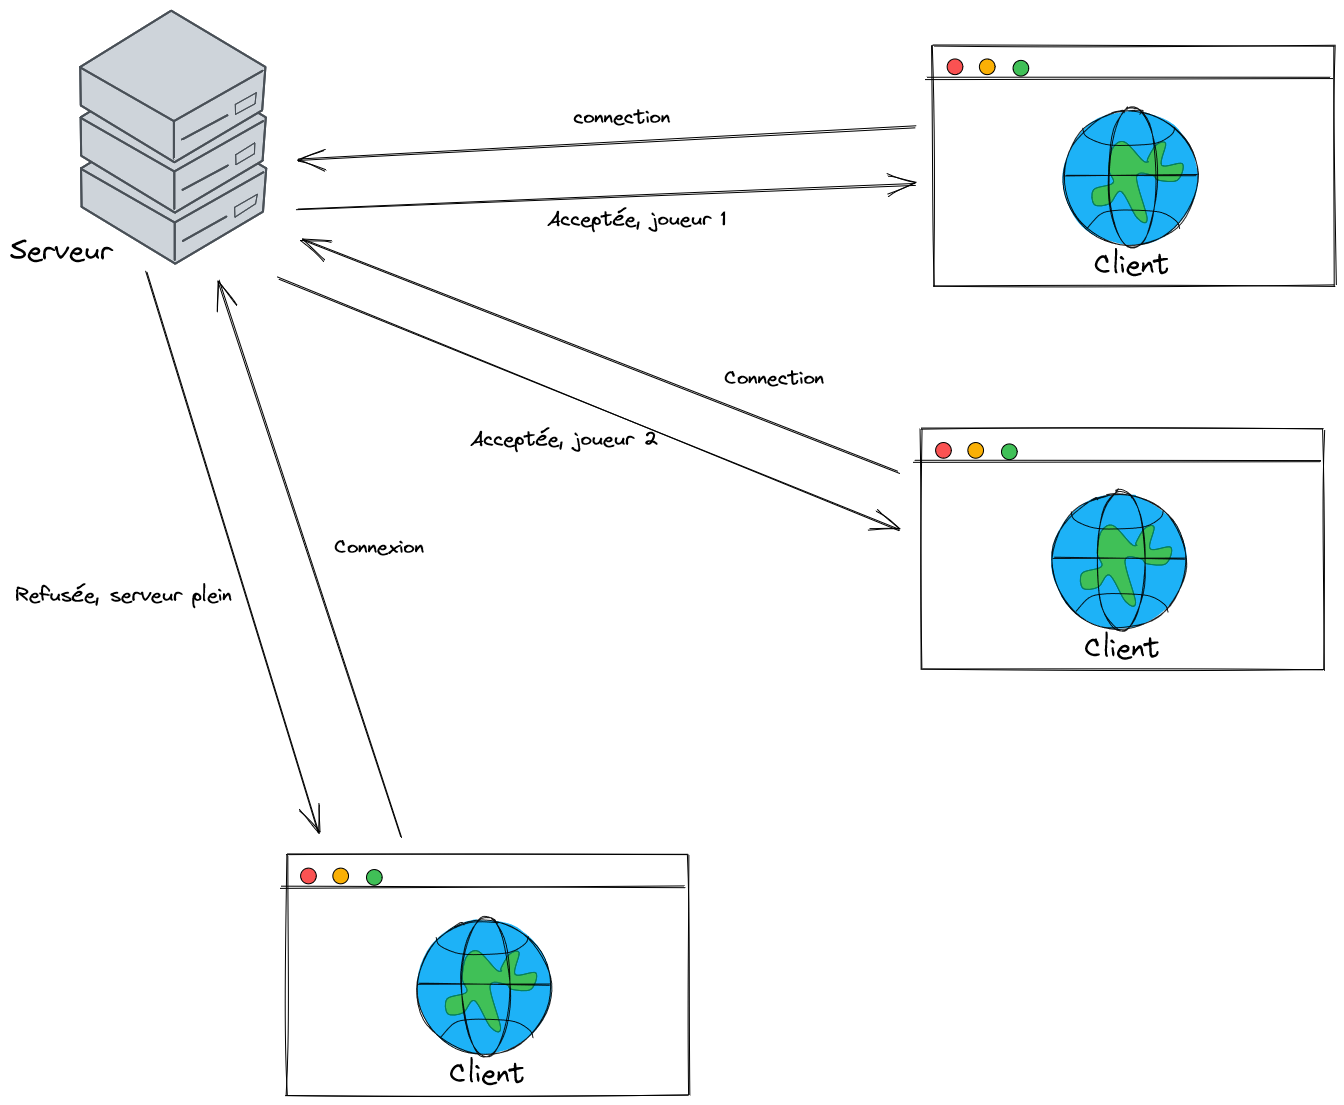
\includegraphics[scale=0.25]{data/reseau_initialisation.png}
    \caption{Phase de connexion des joueurs au serveur}
\end{figure}

Ici on peut voir la première phase du serveur qui permet d'enregistrer les connexions des deux joueurs pour créer une partie.

La partie de connexion est gérée par la bibliothèque {\tt socket-io} que nous utilisons pour le serveur et le client. C'est l'avantage essentiel d'utiliser la même technologie sur le backend et le frontend.

Dans le serveur, nous sauvegardons les sockets qui se connectent au serveur. La limite est de 2 puisqu'il y a 2 joueurs maximum. Quand les 2 joueurs sont bien connectés, la partie est pleine. S'il y en a déjà 2 lors d'une connexion d'un troisième socket, alors la connexion de la troisième est refusée et cette dernière reçoit un code d'erreur, {\tt full}, que le frontend de ce socket va afficher à l'utilisateur.
Si un autre joueur essaie de se connecter, alors le socket n'est pas sauvegardé dans le serveur et elle est déconnectée, il reçoit également une erreur, {\tt full}, qui va s'afficher dans le terminal.

Une fois les deux joueurs créés et la partie initialisée, la carte est envoyée aux deux joueurs pour l'affichage. Voir ci-dessous \ref{reseau_carte}.

\begin{figure}[H]
    \centering
    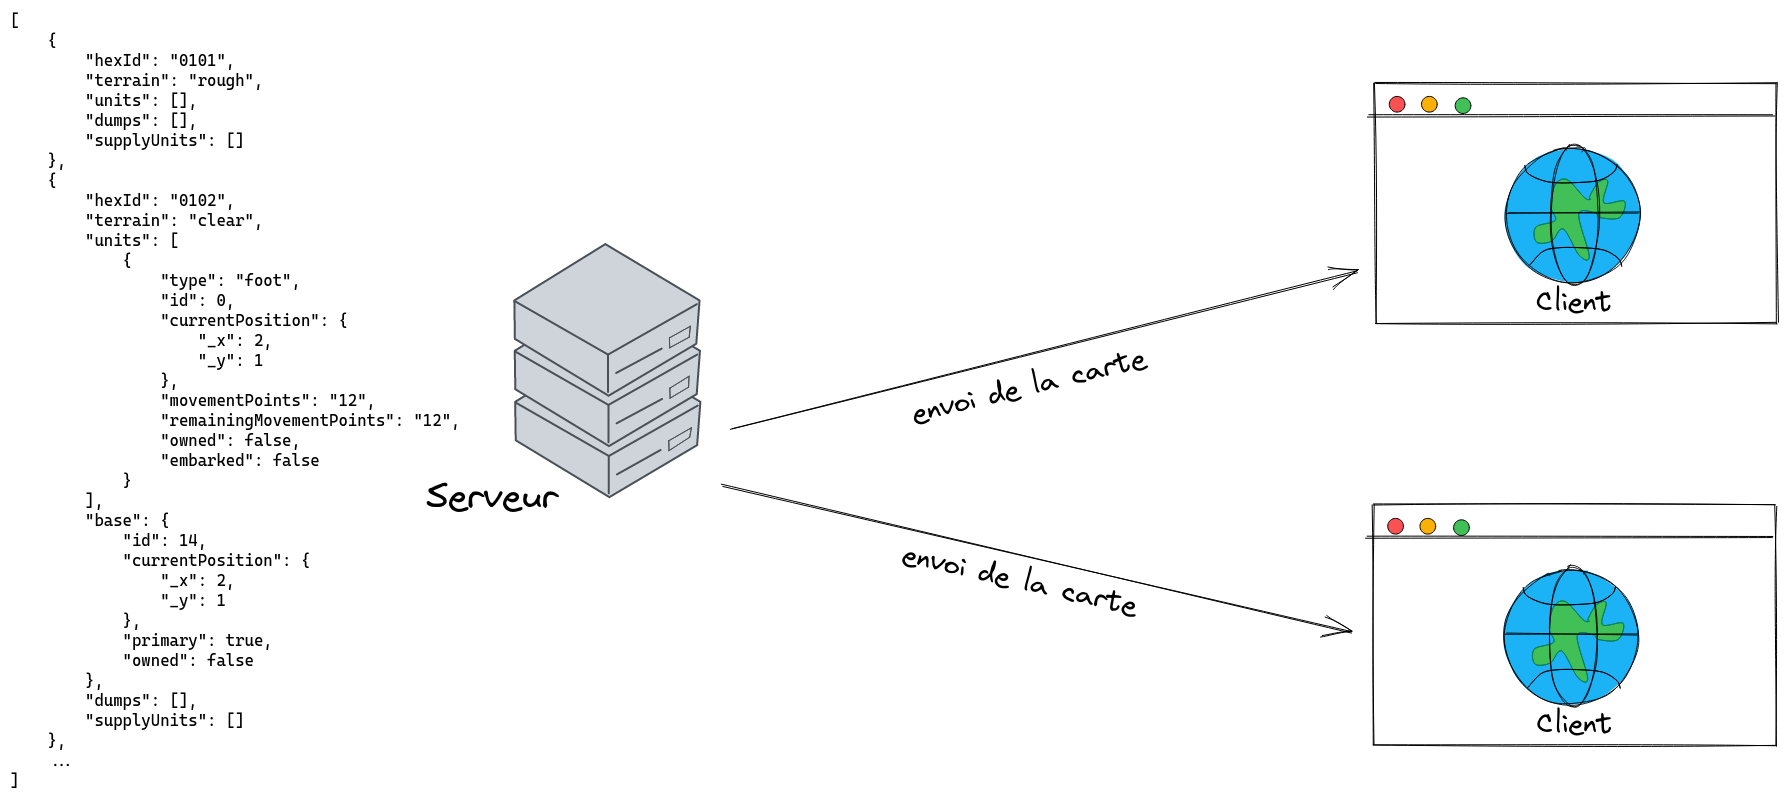
\includegraphics[scale=0.25]{data/reseau_map.png}
    \caption{Phase de connexion des joueurs au serveur}
    \label{reseau_carte}
\end{figure}

Le code à gauche du serveur est le début du {\tt JSON} original envoyé à chaque client.
On peut voir comment il est constitué : c'est un tableau d'objets. Chacun de ces objets représente une case.
Chaque case possède un ``id``, un identifiant, ainsi qu'un ``terrain`` qui décrit son type de terrain.
Il possède aussi 3 aux champs, ``units``, ``dumps`` et ``supplyUnits`` qui sont des tableaux d'objets.
Comme leurs noms l'indique ces objets représentent des tableaux d'unités, de dépôts ou d'unités de ravitaillement.

À partir de ce moment-là, le moteur graphique du jeu est chargé de dessiner la carte reçue en JSON.
L'action \ref{reseau_carte} se répète à chaque changement de la carte dans le jeu.


Les phases vont donc s'enchaîner jusqu'à ce qu'une action d'un joueur soit requise.

\begin{figure}[H]
    \centering
    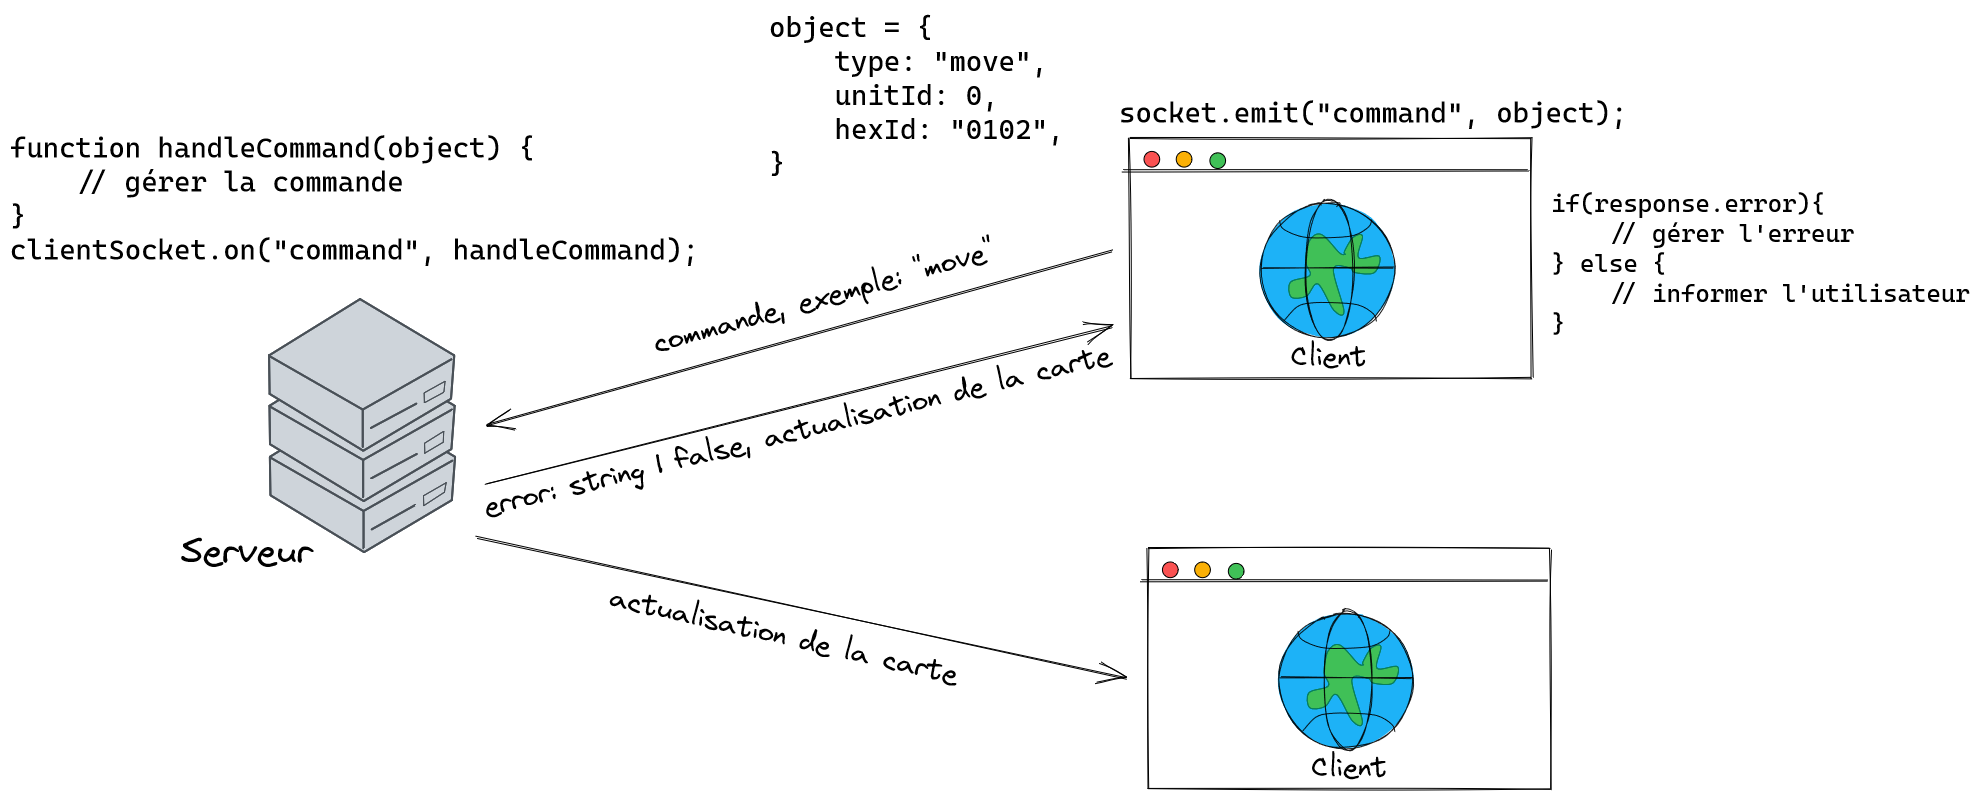
\includegraphics[scale=0.25]{data/reseau_commande.png}
    \caption{Phase de jeu, exemple de commande {\tt move}}
\end{figure}

TODO

La partie s'exécute normalement jusqu'à la fin.

\subsection{Test}

Pour les tests, nous avons utilisé {\tt Mocha} qui est un {\tt framework} de test pour les programmes Node.js.
Nous testons le backend et les communications des sockets parce qu'il est compliqué de tester l'affichage.
Nous avons réalisé des tests unitaires, la couverture ({\tt coverage}) du code est aussi vérifiée grâce à nyc qui est un {\tt framework} compatible avec Mocha.
Nous y reviendrons plus tard dans une partie dédiée.

\subsection{Interface graphique}

Dans le sujet il était indiqué que l'on n'était pas dans l'obligation de faire une interface graphique. Mais afficher un hexagone dans un terminal est compliqué et la moitié de la carte donnée en exemple est de dimensions 32*29 cases, ce qui aurait donné un rendu illisible. Nous avons donc fait le choix de faire une interface graphique. Pour afficher la carte nous avons testé plusieurs bibliothèques et choisis \lstinline{P5.js} pour plusieurs raisons, la documentation est claire et la bibliothèque est plutôt populaire ce qui facilite les recherches lors d'un problème d'implémentation (tutoriels, Stack Overflow...).
Notre approche pour afficher la carte est de la dessiner à chaque changement dans le \lstinline{backend} (exemple: un move). La première raison de cette tactique est de rendre le développement de l'affichage plus facile vu que ce n'est pas la priorité du sujet. Si nous avions dû faire un affichage dynamique il aurait fallu créer des objets pour sauvegarder la position des unités dans chaque case. Ce qui implique alors une duplication de la logique du \lstinline{backend}, nous avons voulu éviter ça. Ici le \lstinline{backend} envoie des données, on les parse et on les affiche.

Pour dessiner les hexagones de la map nous avons cherché des algorithmes pour ne pas avoir à les développer nous-mêmes mais nous n'avons trouvé que des affichages comme suivant.

\begin{figure}[H]
    \centering
    \def\stackalignment{r}
    \stackunder{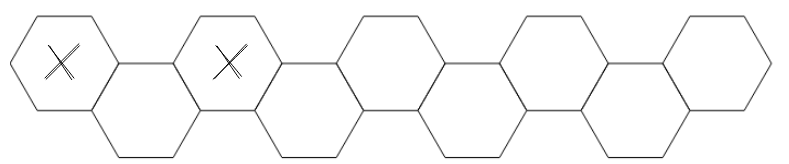
\includegraphics[scale=0.3]{data/hexmap_exemple.png}}%
    {\scriptsize%
        Source : https://eperezcosano.github.io/hex-grid}
    \caption{Deux lignes d'hexagones}
    \label{fig:hexmap_exemple}
\end{figure}

Le problème de ce genre d'affichage est que deux cases sur la même ligne (avec les croix) ne se touchent pas. Si on veut faire un déplacement on doit alors passer par une case intermédiaire dans la ligne au-dessus ou au-dessous, nous voulions éviter ça. Nous avons donc fait nos propres méthodes pour avoir un hexagone dans l'autre sens (avec la pointe vers le haut) et qui est donc adjacente à ses six voisins comme dans la Fig \ref{fig:hexagon}. Pour cela on calcule les points grâce au cercle trigonométrique.



\begin{figure}[H]
    \centering
    \def\stackalignment{r}
    \stackunder{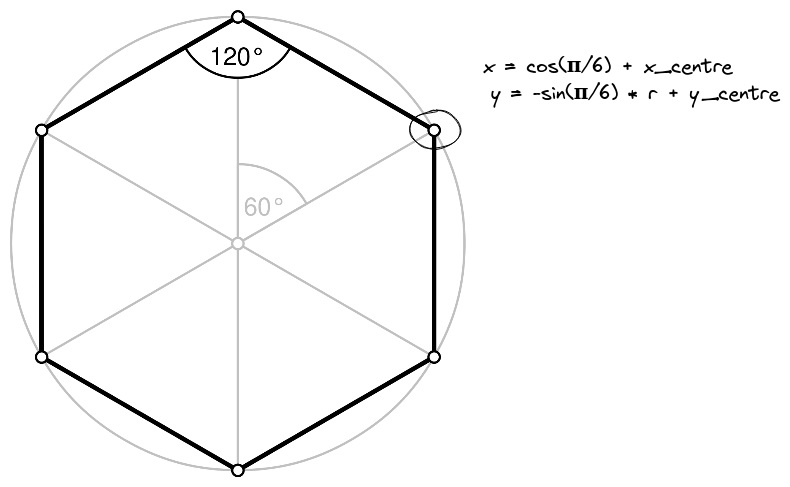
\includegraphics[scale=0.3]{data/hexagon.png}}%
    {\scriptsize%
        Source : https://fr.wikipedia.org/wiki/Hexagone}
    \caption{Les étapes pour dessiner un hexagone}
    \label{fig:hexagon}
\end{figure}

On peut aussi mettre six unités d'attaque dans une case, on réutilise donc le calcul de ces points pour faire la moyenne par rapport au centre. On se retrouve donc avec une unité dans chaque coin de l'hexagone. Ce qui donne le résultat suivant.

\begin{figure}[H]
    \centering
    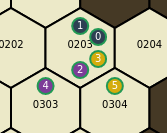
\includegraphics[scale=.7]{data/hexagon_with_units.png}
    \caption{Affichage hexagone avec des unités}
    \label{fig:hexagon_with_units}
\end{figure}